\documentclass[10pt]{Beamer}
\usepackage{fancybox}
\usepackage[most]{tcolorbox}
\usepackage{tikz}
\usepackage[utf8]{inputenc}
\usepackage{graphicx}
\usepackage[utf8]{inputenc}
\usepackage{underscore}

\usetheme{Warsaw}

\title{Impactos da Creche na Primeira Infância: Efeitos Dependendo das Características da Família e do Grau de Exposição ao Centro de Cuidado}
\subtitle{Seminário de Econometria I}

\author{Lorenzo Costa \& Thallyta Marques}
\institute{Universidade Federal do Tocantins}
\date{\today}

\begin{document}
	
\frame{\titlepage}
\frame{\tableofcontents}

\section{Objetivo do Artigo}

\begin{frame}{Objetivo do Artigo}
\begin{block}{}
\begin{itemize}
\item A
\end{itemize}	
\end{block}

\vskip0,5cm

\begin{block}{}
\begin{itemize}
\item B
\end{itemize}	
\end{block}
\end{frame}

\section{Introdução}
\begin{frame}{A Motivação Para o Desenvolvimento do Trabalho}
\end{frame}

\section{As 5 Etapas do Modelo Econométrico}
	
	\subsection{Formulação do Problema}
	
	
\begin{frame}{A Formulação do Problema}
	
\begin{block}{Questão Central}
\begin{itemize}
\item A questão central é como a exposição à creche na primeira infância pode influenciar o desenvolvimento cognitivo e socioemocional das crianças, levando em consideração as características familiares, como a sensibilidade parental, e o grau de envolvimento dos pais. Abordando como esses efeitos variam de acordo com o status socioeconômico familiar.
\end{itemize}
\end{block}
	
\vskip0.5cm
	
\begin{block}{Importância da Formulação do Problema}
\begin{itemize}
\item A formulação do problema destaca a importância de compreender não apenas os efeitos diretos da creche, mas também como esses efeitos são mediados e moderados por fatores familiares e individuais.
\end{itemize}
\end{block}
	
\end{frame}



\begin{frame}{Formulação do Problema}
\begin{tcolorbox}[drop fuzzy shadow=ShadowColor]
- Para as crianças de baixa renda os resultados cognitivos por habilidades de leitura só melhoram se assistem 30 horas por semana, sendo que essa maior exposição ao centro não prejudica a dimensão comportamental. Entretanto, crianças de alta renda não apresentam ganhos cognitivos por passar 30 horas em centros de cuidado e sim experimentam maiores problemas de comportamento.

- Os autores discorrem que crianças pobres devem apresentar maiores benefícios dos centros de cuidado, visto que este deve compensar parcialmente o déficit dos lares.
\end{tcolorbox}

\end{frame}


	\subsection{Bagagem Teórica}
	
\begin{frame}{Bagagem Teórica }
	
\begin{tcolorbox}[drop fuzzy shadow=ShadowColor]
- O consenso da literatura, especialmente de pesquisas não experimentais, tem demonstrado que as experiências em centros de cuidado como nas creches estão relacionadas com melhor desempenho cognitivo das crianças, aumentando os escores em matemática, leitura, vocabulário, linguagem e resolução de problemas em idades da pré-escola e do ensino elementar, comparado com crianças que só tiveram cuidado parental (BELSKY et al., 2007; NICHD, 2006; CLAESSENS, 2012).
	
	
- No caso da dimensão socioemocional, os estudos mostram que o cuidado não parental está associado com maiores níveis de problemas de comportamento externalizantes, que incluem agressividade, hostilidade, raiva e desobediência e parecem ser consistentes em crianças de diferentes países e culturas como Estados Unidos, Austrália e Inglaterra (BELSKY et al., 2007; YAMAUCHI; LEIGH, 2011; HANSEN; HAWKES, 2009; CLAESSENS, 2012).
\end{tcolorbox}	

\end{frame}

\begin{frame}{O Modelo Teórico Conceitual}
	
Os efeitos da creche no desenvolvimento infantil dependem da interação de fatores, como:

\vskip0,5cm


\begin{block}{}
\begin{itemize}
\item[(i)] A qualidade do centro
\end{itemize}	
\end{block}	

\vskip0,5cm

\begin{block}{}
\begin{itemize}	
\item[(ii)] A quantidade ou tempo de exposição
\end{itemize}
\end{block}

\vskip0,5cm

\begin{block}{}
\begin{itemize}	
\item[(iii)] As variáveis da família
\end{itemize}
\end{block}

\end{frame}


\begin{frame}

\shadowbox{A Qualidade do Centro de Cuidado}

\begin{tcolorbox}[drop fuzzy shadow=ShadowColor]
	- Entre os critérios que são consenso na literatura citam-se: i) a relação e interação criança-cuidador, o que é definido como um aspecto de processo; ii) e características estruturais tais como a razão adulto/criança, tamanho das turmas, grau de escolaridade e treinamento sobre aspectos do desenvolvimento infantil (PHILLIPS; LOWENSTEIN, 2011; NICHD, 2006).
\end{tcolorbox}	

\end{frame}

\begin{frame}

\shadowbox{Tempo de Exposição ao Centro de Cuidado}

\begin{tcolorbox}[drop fuzzy shadow=ShadowColor]
	- Sobre o tempo de exposição à creche, os estudos longitudinais têm destacado aspectos como: i) idade de inicio no cuidado; ii) a extensão do cuidado e intensidade (part-time ou full-time) por variáveis como horas por semana ou meses de cuidado ao ano e iii) a estabilidade, ou seja, se há mudanças na frequência ou se há múltiplos usos de centros de cuidado.
\end{tcolorbox}	


\end{frame}

\begin{frame}
	
\shadowbox{Variáveis Familiares}

\begin{tcolorbox}[drop fuzzy shadow=ShadowColor]
- Os efeitos da creche dependem de variáveis familiares estruturais como a renda e o grau de escolaridade materna assim como de aspectos processuais como as práticas e estilos parentais e que determinam as interações e dinâmica familiar.
\end{tcolorbox}	
	
\end{frame}

\begin{frame}

\begin{tcolorbox}[drop fuzzy shadow=ShadowColor]
- Burchinal, Vandell e Belsky (2014) coloca-se a questão de como as experiências em centros de cuidado na primeira infância podem ter efeitos no longo prazo? E como as experiências familiares em distintos momentos do tempo, inclusive posteriores a esse cuidado externo, podem reforçar ou atenuar essas primeiras experiências nos centros de cuidado?

\vskip0.5cm	

- Para responder às questões deve-se considerar que o desenvolvimento humano segue um processo path-dependence, ou seja, experiências em um determinado período levam a uma sequência de resultados em períodos posteriores e, estes por sua vez, influenciam o desenvolvimento em diversas dimensões em idades subsequentes como na adolescência. Masten et al. (2005)
\end{tcolorbox}		
	
	
\end{frame}

	\subsection{Amostragem dos Dados}
	
\begin{frame}{Amostragem dos Dados}
	
\begin{block}{}
\begin{itemize}
	
\item Foram usados dados Pesquisa Longitudinal da Primeira Infância de Chile (ELPI sigla em
espanhol), que contém uma amostra de 5.623 crianças de 4 a 5 anos cujas avaliações no desenvolvimento foram realizadas nessa idade, mas que se relacionam com o acumulativo de meses de assistência à creche quando elas tinham 0 a 3 anos e 11 meses de idade. Assim, a análise é de corte transversal (cross-section) usando dados das avaliações de 2012 (segunda rodada da pesquisa longitudinal).  

\item A pesquisa contém informações retrospectivas de assistência a centros de cuidado em intervalos de idade da criança. Esses intervalos são: de 0 a 3 meses, 3 a 6 meses, 6 a 12 meses, 12 a 18 meses, 18 a 24 meses, de 2 a 3 anos e de 3 a 4 anos. Assim, o grau de exposição à creche é medido pela soma dos meses reportados de assistência à creche em todos esses intervalos de tempo.
	
\end{itemize}
\end{block}	
	
\end{frame}

\begin{frame}

\begin{block}{Teste de Vocabulário em Imagens (TVIP)}
\begin{itemize}
\item usado para inferir sobre a inteligência  verbal, a compressão narrativa da criança, parte da competência intelectual e também pode ser usado como indicador preditivo do sucesso escolar. 
\end{itemize}
\end{block}

\begin{block}{Tests Child Behavior Checklist (CBCL)}
\begin{itemize}
\item afere problemas de comportamentos emocionais das crianças tanto internalizantes como externalizantes.
\end{itemize}
\end{block}

\end{frame}

\begin{frame}



\begin{tcolorbox}[drop fuzzy shadow=ShadowColor]
- A dimensão socioemocional da mãe é avaliada por subáreas de neuroticismo, amabilidade e extroversão  do “Big Five Inventory”. Para avaliar o ambiente familiar construíram-se indicadores normalizados em uma escala de 0 a 1 sobre práticas de envolvimento parental, sensibilidade materna, exercício de disciplina coercitiva e a presença de recursos de aprendizagem no lar

\vskip0.5cm

- A sensibilidade parental é um indicador construído com base no Inventario HOME (Home
Observation for Measurement of the Environment), o qual representa a sensibilidades materna em direção à criança em termos de afetividade, orgulho e ternura. As questões usadas registram se a mãe anima, elogia ou faz carinho à criança assim como se responde rapidamente e adequadamente às necessidades dela.
\end{tcolorbox}


\end{frame}

\begin{frame}{Variáveis do Modelo e Medição}
	
	
	\begin{figure}[b]
		\centering
		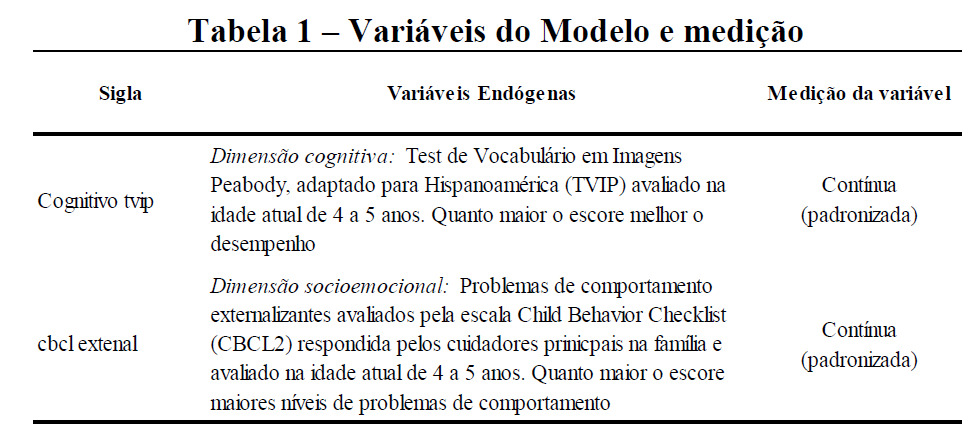
\includegraphics[width=1.0\textwidth]{endo}
	\end{figure}
	
\end{frame}

\begin{frame}
	
	\begin{figure}[b]
		\centering
		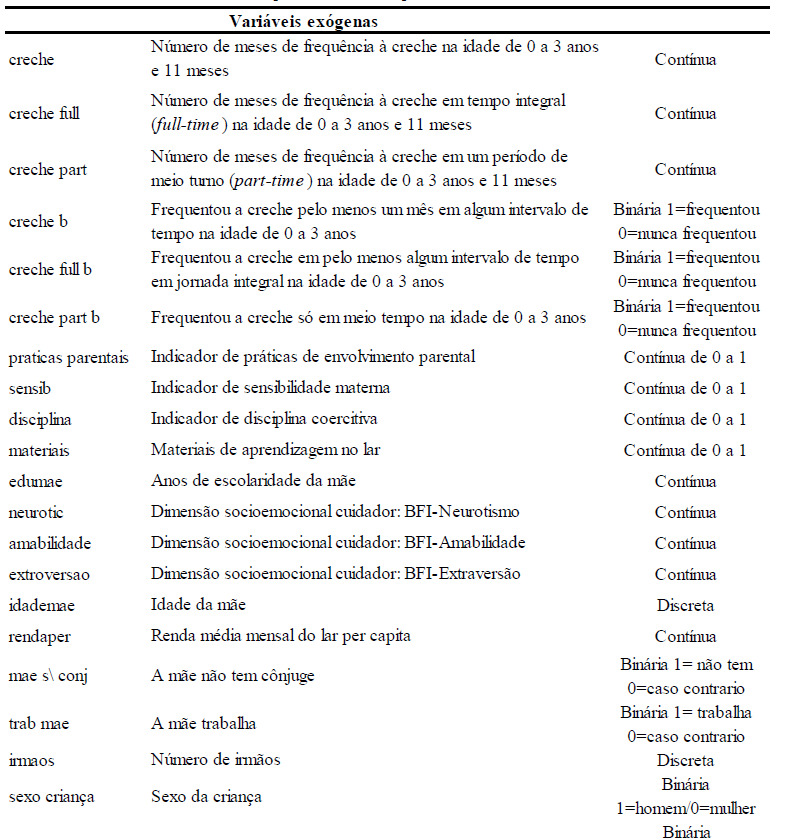
\includegraphics[width=0.6\textwidth]{exo1}
	\end{figure}
	
\end{frame}

\begin{frame}
	
	\begin{figure}[b]
		\centering
		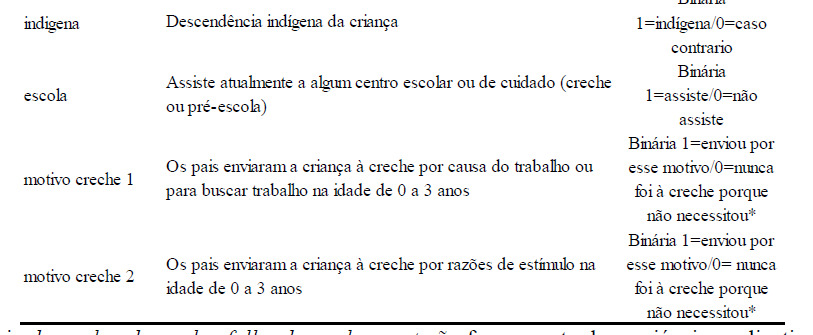
\includegraphics[width=1.0\textwidth]{exo2}
	\end{figure}
	
\end{frame}	
	


	\subsection{Modelo Econométrico}

\begin{frame}{O Método e a Regressão Linear Múltipla}
	
\shadowbox{Structural Equation Modeling - SEM}	

\begin{figure}[h]
	\centering
	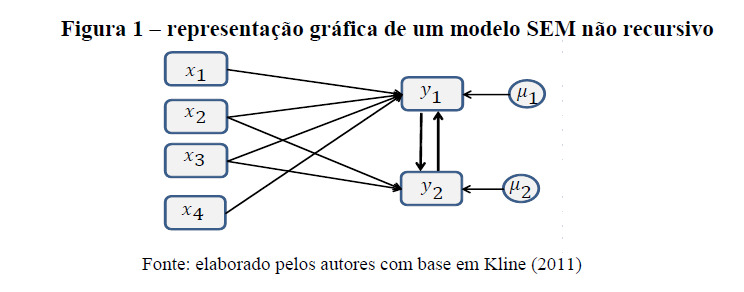
\includegraphics[width=0.8\textwidth]{SEM}
\end{figure}

\end{frame}

\begin{frame}{As Regressões}	


\begin{block}{}
\begin{itemize}
\item A equação básica do sistema de regressões é a seguinte: 
\end{itemize}
\end{block}


\begin{equation}
Y_{1i} = \alpha_1Y_{2i} + \beta_1creche_i + \beta_2familia_i + \beta_3criança_i + \beta4motivocrechei + \mu_i
\end{equation}

\begin{equation}
Y_{2i} = \alpha_1Y_{1i} + \beta_1creche_i + \beta_2familia_i + \beta_3criança_i + \beta_4motivocrechei + \mu_i
\end{equation}

\begin{tcolorbox}[drop fuzzy shadow=ShadowColor]
Em que $Y_{1i}$ representa o desempenho cognitivo ($cognitivo tvip$) e $Y_{2i}$ são os problemas externalizantes
\end{tcolorbox}

\end{frame}
	
\begin{frame}{As Regressões}

\begin{itemize}
\begin{block}
\item As equações que incluem as interações mencionadas e que permitirá verificar as diferenças dos efeitos da creche são:
\end{block}
\end{itemize}

\begin{equation}
Y_{1i} = \alpha_1Y_{2i} + \beta_1creche_i + \beta_2edumae_i + \beta_3creche.edumae_i + \beta_4familia_i \\ + \beta_5criança_i + \beta_6motivocreche_i + \mu_i
\end{equation}

\begin{equation}
Y_{1i} = \alpha_1Y_{2i} + \beta_1creche_i + \beta_2praticas_i + \beta_3creche.praticas_i + \beta_4familia_i \\ + \beta_5criança_i + \beta_6motivocreche_i + \mu_i
\end{equation}

\begin{equation}
Y_{1i} = \alpha_1Y_{2i} + \beta_1creche_i + \beta_2sens_i + \beta_3creche.sensib_i + \beta_4familia_i \\ + \beta_5criança_i + \beta_6motivocreche_i + \mu_i
\end{equation}

\end{frame}

\subsection{Mensuração e Análise}
	
	
\begin{frame}{Estatísticas Descritivas}

\begin{figure}[h]
\centering
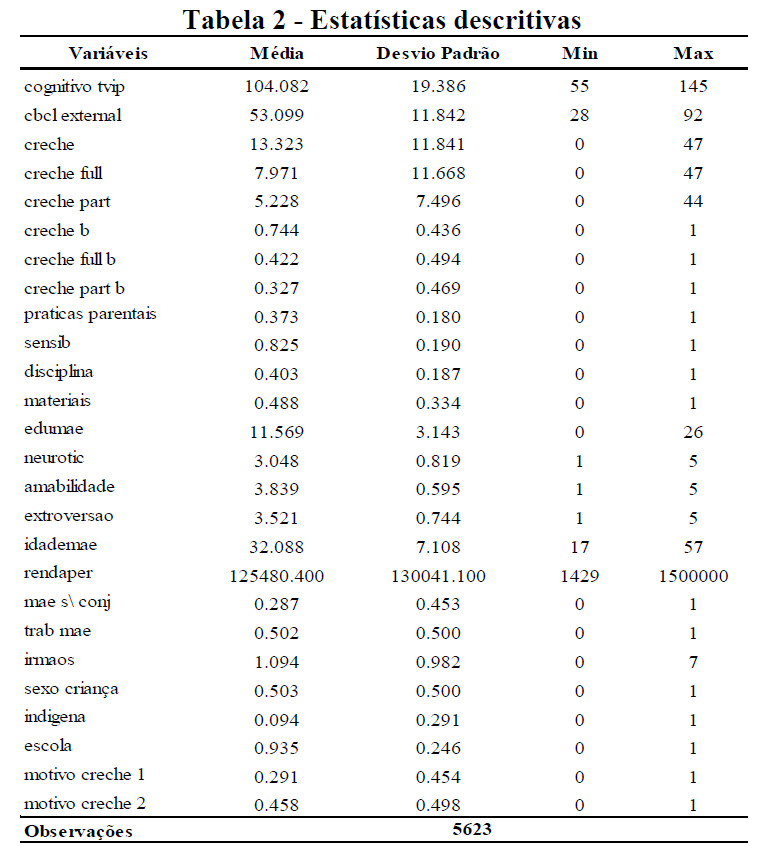
\includegraphics[width=0.8\textwidth]{estat}
\end{figure}
	
\end{frame}

\begin{frame}{Resultado das Regressões}
\shadowbox{Tabela 3 - Desempenho Cognitivo}

\begin{figure}[h]
\centering
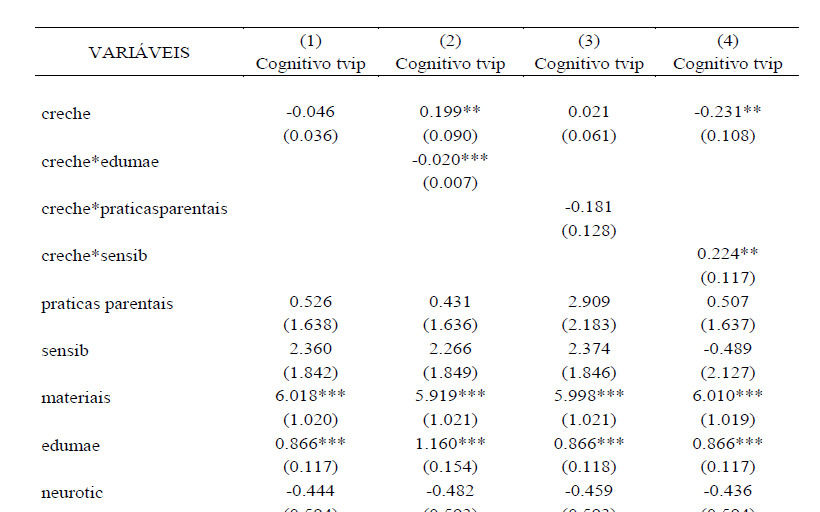
\includegraphics[width=1.0\textwidth]{Tab3}
\end{figure}

\end{frame}

\begin{frame}{Resultado das Regressões}
\shadowbox{Tabela 4 - Efeitos Externalizantes}
	
\begin{figure}[h]
\centering
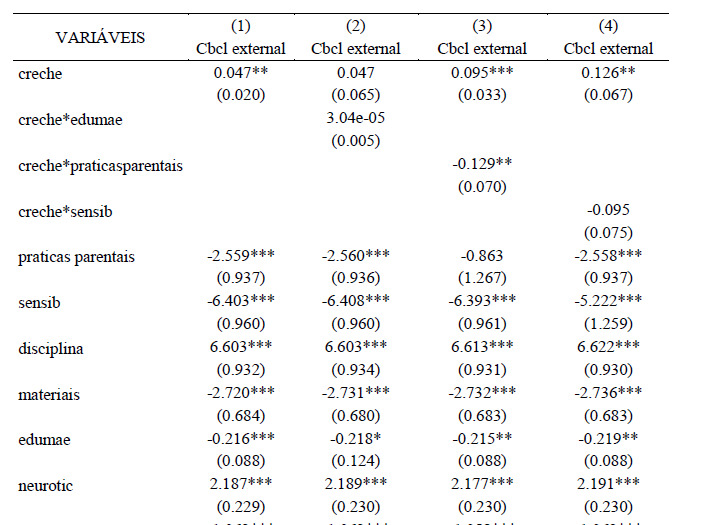
\includegraphics[width=1.0\textwidth]{Tab4}
\end{figure}
	
\end{frame}

\begin{frame}{Resultado das Regressões}
\shadowbox{Tabela 5 - Desempenho Cognitivo full time e part time}
	
\begin{figure}[h]
\centering
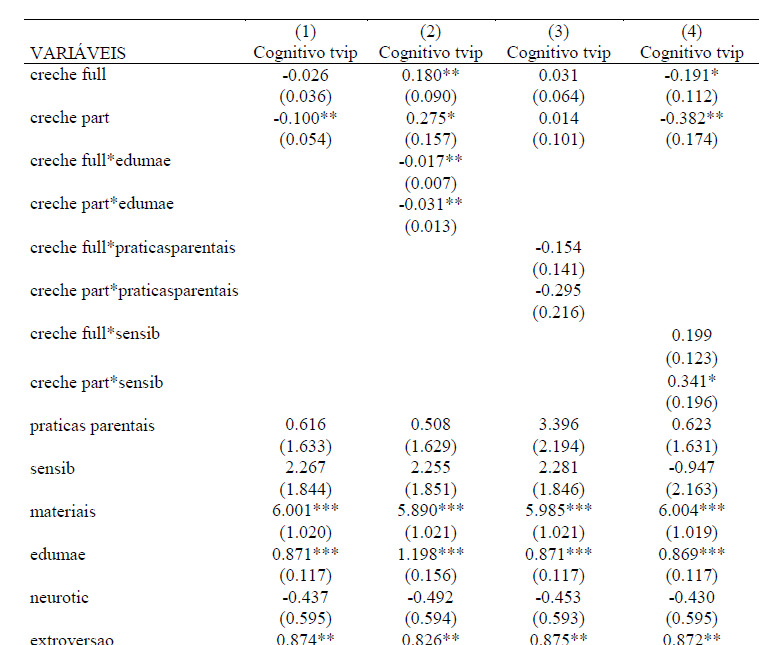
\includegraphics[width=1.0\textwidth]{Tab5}
\end{figure}
	
\end{frame}

\begin{frame}{Resultado das Regressões}
\shadowbox{Tabela 6 - Efeitos Externalizantes full time e part time}
	
\begin{figure}[h]
\centering
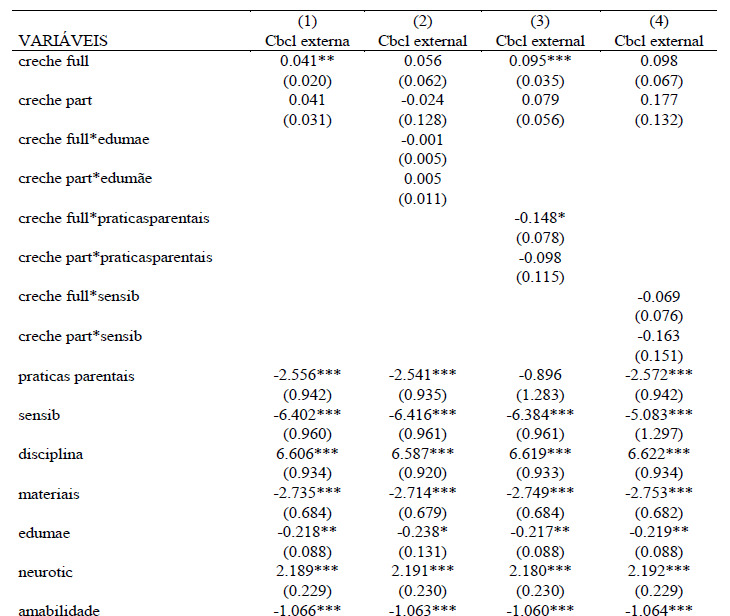
\includegraphics[width=1.0\textwidth]{Tab6}
\end{figure}
	
\end{frame}
	
\end{document}